\begin{refsection}

\hypertarget{introduction-guxe9nuxe9rale}{%
\chapter{Introduction Générale}\label{introduction-guxe9nuxe9rale}}

L'écologie est une science multidisciplinaire, qui a subi des
développements rapides au cours des dernières décennies et dont le but
est de comprendre la contribution relative des facteurs biotiques et
abiotiques sur la dynamique spatio-temporelle de la biodiversité
\autocite{Campbell_2012}. Ces patrons de biodiversité peuvent s'étudier
à des échelles différentes, qui peuvent être grandes comme les forêts
tropicales ou la mer \autocite{Chapin_2011}, ou à des échelles plus
locales, par exemple le microbiome intestinal \autocite{Foster_2017}. La
biodiversité peut se mesurer à différents niveaux d'organisation allant
de l'individu à l'écosystème en passant par les espèces, les populations
ou les communautés. Différentes méthodes existent pour décrire et
comprendre les patrons de biodiversité et ont donné lieu à la création
de nouvelles sous-disciplines comme l'écologie expérimentale, l'écologie
des communautés ou l'écologie quantitative.

Les premiers naturalistes qui contribuèrent au développement de
l'écologie ont tout d'abord adopté une approche descriptive en voyageant
à travers le monde et en collectant des spécimens végétaux et animaux
comme l'on fait \textcite{Linnaeus_1789}, \textcite{Humboldt_1805},
\textcite{Darwin_1839} et bien d'autres encore. Pendant leurs voyages,
ces pionniers de l'écologie ont été fascinés par les différences dans le
nombre d'espèces pouvant coexister dans différentes parties de globe.
Ces patrons de diversité observés ont généré un ensemble de questions
macroécologiques auxquelles il était difficile de répondre à cause du
manque de données à l'échelle du globe et de moyens de les analyser.
Ainsi, bien que des hypothèses furent développées rapidement pour
expliquer les variations de biodiversité observée, ces dernières étaient
difficilement testables. Pendant longtemps, les écologues ne purent
s'intéresser qu'à des échelles spatiales et temporelles restreintes et
tester des hypothèses sur les patrons de distribution des espèces à des
échelles locales. Grâce aux développements technologiques permettant de
collecter toujours plus de données à des résolutions toujours plus fines
et à des échelles spatio-temporelles toujours plus importantes, par
exemple avec les apports de la télédétection ou les développements de la
biologie moléculaire \autocite{Edgar_2016} et l'apport d'outils
numériques et de modélisation \autocites[ ]{Legendre_2012}{Guisan_2017},
les chercheurs ont pu développer de nouvelles hypothèses et théories
pour expliquer les patrons de diversité observée sur notre planète (voir
par exemple \textcite{Hubbell_2001}, \textcite{Vellend_2017} ou bien
encore \textcite{Leibold_2018}).

Cette thèse s'inscrit dans un des sous-domaines de l'écologie qui est
celle de l'écologie des communautés. L'écologie des communautés
s'intéresse aux communautés, c'est-à-dire aux espèces vivant
interagissant entre elles de manière directe ou indirecte, même endroit
et au même moment \autocite{Vellend_2017}. Ce champ de recherche vise à
identifier les règles générales qui régissent les patrons de diversité,
l'abondance et la composition en espèces des communautés
\autocite{Vellend_2010}.

Lors de l'émergence de ce champ disciplinaire, les chercheurs se sont
intéressés tout d'abord à étudier les règles d'assemblage des espèces
autour du prisme des interactions biotiques et particulièrement
trophiques ou bien en se concentrant sur les facteurs abiotiques et les
gradients environnementaux \autocite{Whittaker_1975}. Ces études se
firent tout d'abord sur des échelles spatiales limitées
\autocite{Whittaker_1960}. A l'ère du numérique, la collecte massive de
données à de plus grandes échelles spatiales et l'application des outils
de l'écologie quantitative nous permettent de mieux prendre en compte
l'importance relative de ces différents facteurs \autocite{Gaston_2000}.
Dans le cadre de cette thèse, et en m'appuyant sur des jeux de données
collectées à plus ou moins larges échelles spatiales et temporelles, je
vais essayer de comprendre en appliquant certains des outils, des
techniques et méthodes de l'écologie quantitative, comment les habitats
benthiques biogéniques structurent la diversité des communautés des
écosystèmes marins côtiers et comment ils répondent face aux changements
environnementaux et anthropiques, afin de mieux appréhender le futur des
écosystèmes marins côtiers face aux changements globaux.

\hypertarget{uxe9cosystuxe8mes-cuxf4tiers}{%
\section{Écosystèmes Côtiers}\label{uxe9cosystuxe8mes-cuxf4tiers}}

\hypertarget{uxe9cosystuxe8mes-cuxf4tiers-biodiversituxe9-et-enjeux-humains}{%
\subsection{Écosystèmes Côtiers : Biodiversité et Enjeux
Humains}\label{uxe9cosystuxe8mes-cuxf4tiers-biodiversituxe9-et-enjeux-humains}}

À la croisée des milieux terrestres et marins, les écosystèmes côtiers
sont des écosystèmes abritant une grande biodiversité
\autocite{ippc_chap6}. Cette biodiversité est supportée par la variété
d'habitats que comprennent les écosystèmes côtiers
(Fig.~\ref{fig:intro1}). Côté terre, on trouve des zones urbaines,
industrielles, mais également des espaces naturels comme les falaises ou
les dunes \autocite{Burke_2000}. Côté mer, ces écosystèmes comprennent
des milieux intertidaux tels que les plages, les estuaires et les
lagons, ainsi que des milieux subtidaux comme les forêts de laminaires
ou les récifs coralliens \autocite{Burke_2000}, qui sont parmi les
milieux abritant une des plus grandes biodiversité et productivité au
monde \autocite{Wernberg_2023}.

\begin{figure}
\hypertarget{fig:intro1}{%
\centering
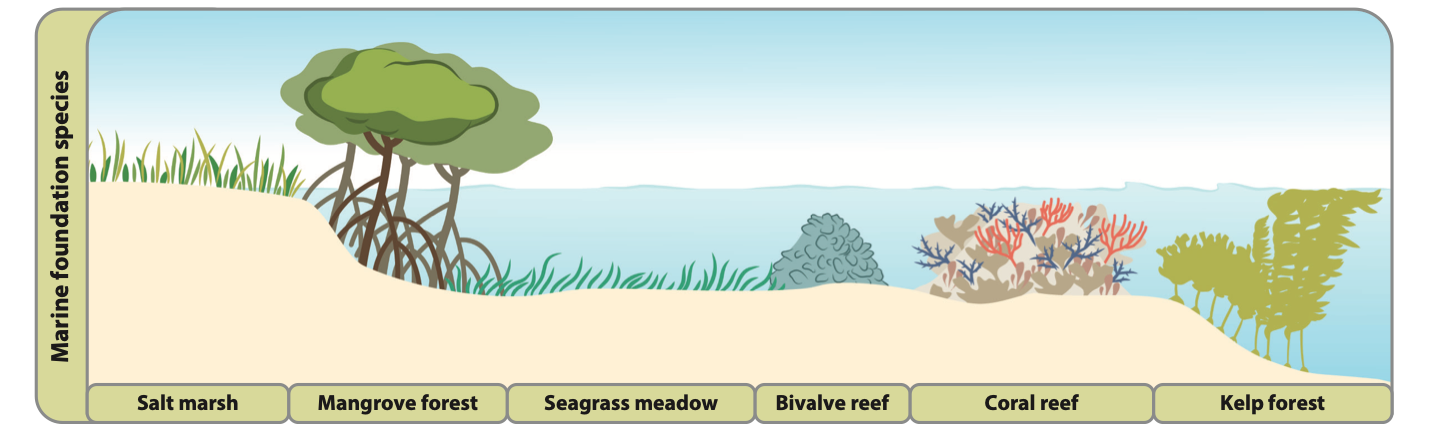
\includegraphics{02-Introduction/figures/Marine_Habitat_list.png}
\caption[Illustration du continuum terre-mer et des différents habitats
marins qu'abritent les écosystèmes côtiers]{Illustration du continuum terre-mer et des différents habitats
marins qu'abritent les écosystèmes côtiers. De gauche à droite : Pré
salé, Mangrove, Herbier marin, Récif de bivalves, Récif corallien, Forêt
de laminaires. Illustration \textcite{Wernberg_2023}}\label{fig:intro1}
}
\end{figure}

Parallèlement à leur importance écologique, les régions côtières jouent
un rôle crucial dans la dynamique des populations humaines. En effet,
65\% des mégalopoles de la planète sont situées sur les côtes
\autocite{Blackburn_2019}. Actuellement, près de 40\% de la population,
soit 2,8 milliards d'individus, vivent dans un rayon de 100 km autour
des côtes \autocite{Maul_2019}. Si ce pourcentage devrait rester stable
jusqu'en 2035, la population côtière devrait néanmoins augmenter de 355
millions d'habitants au cours des quinze prochaines années
\autocite{Maul_2019}. Cette concentration démographique illustre
l'importance cruciale des zones côtières pour le développement
socio-économique dans les décennies à venir, mais cette concentration
démographique implique également des pressions importantes sur les
écosystèmes côtiers.

En somme, les écosystèmes côtiers, en plus d'être d'une forte richesse
écologique, sont au cœur d'enjeux démographiques et socio-économiques.
Leur préservation et leur gestion durable sont essentielles, non
seulement au regard de la biodiversité qu'ils abritent, mais aussi pour
l'avenir des populations humaines qui en dépendent.

\hypertarget{contribution-des-uxe9cosystuxe8mes-cuxf4tiers-aux-services-uxe9cosystuxe9miques}{%
\subsection{Contribution des Écosystèmes Côtiers aux Services
Écosystémiques}\label{contribution-des-uxe9cosystuxe8mes-cuxf4tiers-aux-services-uxe9cosystuxe9miques}}

Notre planète est recouverte à 71\% par les océans ; or les zones
côtières définies par la limite du plateau continental ne représentent
qu'environ 9\% de la superficie des océans \autocite{Harris_2014}.
Cependant, cette zone abriterait y abriterait selon les estimations,
près de 91 \% de la biodiversité \autocite{Costello_2017}. Cette forte
biodiversité soutient un éventail de services écosystémiques essentiels
aux populations humaines. Ces services peuvent être classés en
différentes catégories : les services de régulation, les services
d'approvisionnement et les services culturels (\textcite{Reid_2005} ;
Fig.~\ref{fig:intro2}).

Les services d'approvisionnement sont les plus simples à définir. Ce
sont les services écosystémiques qui fournissent des ressources à l'être
humain comme de la nourriture ou bien des matériaux. Par exemple, les
petites pêcheries côtières capturent environ 25 millions de tonnes de
poissons par an \autocite{Cochrane_2023} et 90\% des espèces ciblées par
la pêche \autocite{FAO_yearbook_2022}. De même, les pêcheries de
crustacés et de coquillages ainsi que leurs élevages représentent des
secteurs commerciaux importants avec respectivement, près de 17 millions
et 24 millions de tonnes \autocite{FAO_yearbook_2022}. Les écosystèmes
côtiers constituent également un réservoir important en termes de
ressources médicinales. De nombreux organismes tels que les algues,
oursins ou hippocampes entrent dans la composition de médicament : par
exemple, dans celle de nombreuses médecines traditionnelles \autocites[
]{Kumaravel_2012}[ ]{Thurstan_2018}{Sibiya_2021}, mais également en
médecine moderne avec par exemple l'isolement de composés anticancéreux
\autocite{Schwartsmann_2001}, antiviraux \autocite{Yasuhara-Bell_2010},
antibiotiques \autocite{Benoist_2020} ou antidouleurs
\autocite{Miljanich_2004}.

Les écosystèmes marins côtiers offrent un nombre de services
immatériels, souvent encapsulés dans la terminologie des services
culturels, qui englobent une gamme diversifiée de bénéfices que
l'humanité tire directement ou indirectement de ces écosystèmes. L'un
des aspects les plus manifestes réside dans l'esthétisme des paysages
marins, qui inspirent l'art, la littérature et d'autres expressions
culturelles \autocite{Ghermandi_2010}. Parallèlement, la biodiversité et
la beauté naturelle de ces régions stimulent des activités
récréationnelles et constituent un moteur essentiel du tourisme côtier.
Les écosystèmes côtiers sont aussi au centre des cultures et des
spiritualités qu'entretiennent les populations côtières avec leur
environnement marin. En effet, pour de nombreuses populations, la mer
n'est pas simplement un élément géographique, mais un pilier de leur
patrimoine culturel et de leur histoire collective
\autocite{Ghermandi_2010}.

Les services de régulation sont eux moins visibles, puisqu'ils
rassemblent tous les processus qui permettent de maintenir notre
environnement dans des conditions stables. Par exemple, les écosystèmes
côtiers participent à la régulation de la qualité de l'eau, en piégeant
des polluants dans les écosystèmes estuariens \autocite{Barbier_2011} ou
en protégeant le trait de côte des vagues et de l'érosion à l'aide des
récifs coralliens, des prés-salés ou bien des forêts de mangroves
\autocites[ ]{Barbier_2011}{Harris_2018}. Les herbiers marins et les
forêts de laminaires offrent également d'autres services en permettant
notamment de moduler les effets du changement climatique global en
agissant comme des puits de carbones \autocites[
]{Fourqurean_2012}{Filbee-Dexter_2018}.

La valeur économique des services produits par les écosystèmes est
toutefois dépendante de leur état de santé \autocite{Sutton_2016}. Or
plus de 75\% des écosystèmes terrestres et 66\% des écosystèmes marins
sont dégradés \autocite{ipbes_2019}. Cette dégradation conduit à une
réduction drastique de la capacité des écosystèmes à fournir des
services essentiels et à soutenir les activités économiques qui en
dépendent \autocite{ipbes_2019}. Ainsi, la préservation et la
restauration des écosystèmes deviennent non seulement un impératif
écologique et économique, mais sont aussi essentielles pour le bien-être
et la santé des populations humaines. Assurer leur durabilité est
primordial pour garantir la pérennité des bénéfices socio-économiques
qu'ils procurent à l'humanité \autocite{ipbes_2019}.

\begin{figure}
\hypertarget{fig:intro2}{%
\centering
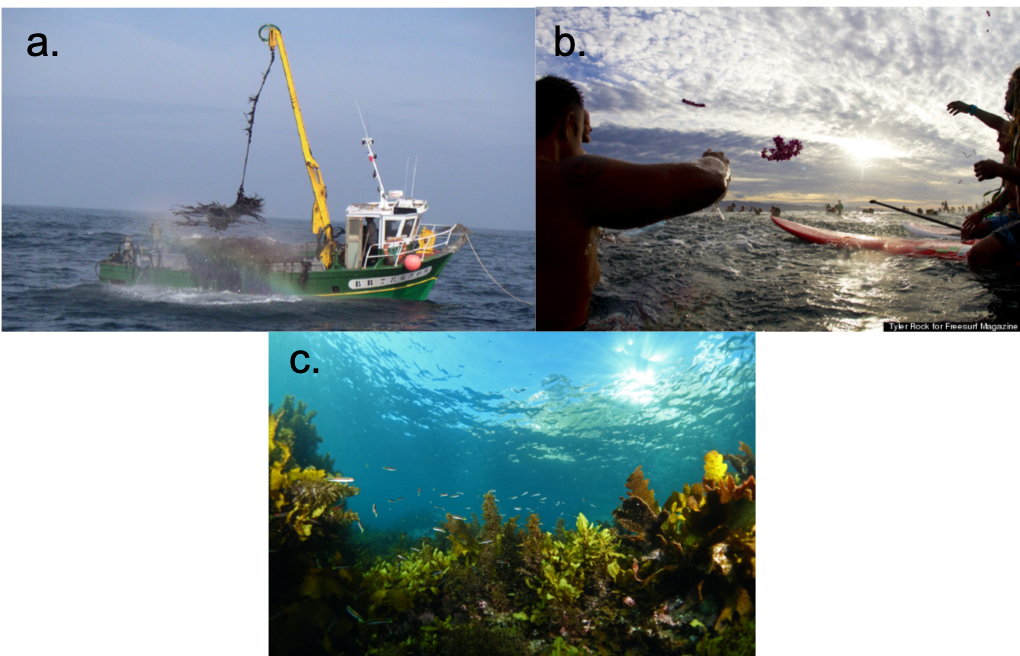
\includegraphics{02-Introduction/figures/ecosystem_services.png}
\caption[Illustration de services écosystémiques fournis par les océans]{Illustration de services écosystémiques fournis par les océans.
a. Cueillette de \emph{Laminaria digitata} en mer d'Iroise. b. Cérémonie
du \emph{Paddle-out}. c.~Forêt de laminaires et de fucoïdes contribuant
à différents services de régulation. © Image: a. Agrocean. b. Tyler
Rock, Freesurf Magazine. c.~John Turnbull}\label{fig:intro2}
}
\end{figure}

\hypertarget{les-uxe9cosystuxe8mes-cuxf4tiers-face-aux-pressions-anthropiques}{%
\subsection{Les Écosystèmes Côtiers face aux Pressions
Anthropiques}\label{les-uxe9cosystuxe8mes-cuxf4tiers-face-aux-pressions-anthropiques}}

Le rôle majeur de l'espèce humaine dans la transformation de notre
planète n'est maintenant plus à démontrer. Notre impact est tellement
significatif que les géologues proposent de désigner notre époque
actuelle comme l'Anthropocène \autocite{Subramanian_2019}. Ce nouvel âge
géologique est symbolisé par la libération massive de CO\(_2\) dans
l'atmosphère. Plus de 555 milliards de tonnes depuis la première
révolution industrielle ont été relâchées \autocite{Lewis_2015},
entraînant un changement climatique global \autocite{Calvin_2023}. Face
à ce bouleversement, la biosphère, et notamment les écosystèmes côtiers,
se retrouve grandement perturbée. Les modifications que nous observons
aujourd'hui, liées aux activités humaines \autocite{Calvin_2023},
peuvent être classées en deux types d'impacts : directs et indirects.

La plupart des pressions exercées sur les écosystèmes côtiers découlent
de l'augmentation de la densité de population côtière. La densification
de la population humaine le long des côtes entraîne de nombreuses
perturbations, par exemple des ruissellements urbains qui sont source de
différentes pollutions que ce soit aux métaux lourds ou en polluants
organiques ou plastiques \autocite{Todd_2019}. A ces pollutions
facilement identifiables s'ajoutent celles liées au bruit ou à la
lumière \autocite{Todd_2019}. Ces dernières peuvent modifier le
comportement de nombreuses espèces \autocite{Todd_2019} et entraîner des
modifications plus ou moins profondes des communautés. Par exemple, les
efflorescences d'algues causées par l'eutrophisation peuvent entraîner
la mort de nombreux organismes comme des poissons, crustacés ou bien
mollusques \autocite{Todd_2019}. Ces efflorescences ont également un
fort impact économique sur les zones littorales souvent lié entre autres
à une diminution de l'activité touristique, à des impacts sur la santé
humaine et sur les pêcheries \autocite{EuropeanCommission_2016}.

L'accroissement des activités humaines liées à l'usage de l'espace
côtier entraîne également d'autres menaces, par exemple la prolifération
d'espèces non indigènes envahissantes, souvent introduites par des
navires en transit dans différents ports \autocite{Hardiman_2010}.
Attachées aux coques des navires, ou contenue dans l'eau des ballastes
de plus gros navires, des espèces non indigènes animales comme végétales
ainsi que de nouveau pathogènes peuvent être introduits dans de
nouvelles zones géographiques \autocite{Hardiman_2010}.

D'autres impacts anthropiques directs viennent de l'exploitation des
ressources des espaces maritimes côtiers. Ainsi, les ressources
halieutiques sont largement exploitées : près de 65\% des espèces
commerciales sont exploitées à leur niveau maximal alors que 35\% des
espèces sont surexploitées \autocite{FAO_yearbook_2022}. L'extraction
d'autres ressources comme le sable, utilisé pour la construction et
extrait via des opérations de dragage, impacte également fortement les
écosystèmes côtiers, en particulier les écosystèmes benthiques
\autocites[ ]{Boyd_2003}[ ]{Boyd_2005}{Erftemeijer_2006}. Au-delà de ces
impacts directs, les opérations de dragage peuvent modifier la
bathymétrie et les courants \autocite{Bray_2008}, remettent en
suspensions des sédiments dans la colonne d'eau
\autocite[@][]{Erftemeijer_2006}, et relarguent un certain nombre de
polluants \autocite{Filho_2004}.

L'impact anthropique indirect sur les écosystèmes est, quant à lui,
principalement dû au changement climatique global, lié aux émissions de
gaz à effet de serre (CO\(_\text{2}\) et CH\(_\text{4}\) en
particulier), avec un réchauffement de l'océan compris entre 0.68 et
1.01 °C depuis l'ère préindustrielle \autocite{ipcccryosphere_2021}.
Conjointement avec l'augmentation globale des températures moyennes de
l'eau de surface, on observe une augmentation en fréquence, en durée et
en intensité d'événements climatiques marins extrêmes, tels que les
vagues de chaleur marine \autocite{Oliver_2018} ou les tempêtes. Ces
vagues de chaleur sont l'équivalent des canicules terrestres et se
produisent tant en zones tempérées que tropicales
(\textcite{Hobday_2016} ; Fig.~\ref{fig:intro3}). Elles ont, par
exemple, entraîné des vagues de blanchissement des coraux et une
augmentation de leur mortalité autour de Moorea en 2019
\autocite{Wyatt_2023} ou encore la disparition de forêts de laminaires
le long de la côte ouest-australienne \autocite{Wernberg_2016}. Les
prédictions du \emph{GIEC} font état d'une augmentation de 4 à 8 fois de
la fréquence des vagues de chaleur en fonction des scénarios de
réduction des émissions de gaz à effet de serre
\autocite{ipcccryosphere_2021}. Ainsi l'impact de ces canicules marines
sur les écosystèmes marins devrait augmenter dans les années à venir
\autocites[ ]{Oliver_2018}{Smith_2023}.

\begin{figure}
\hypertarget{fig:intro3}{%
\centering
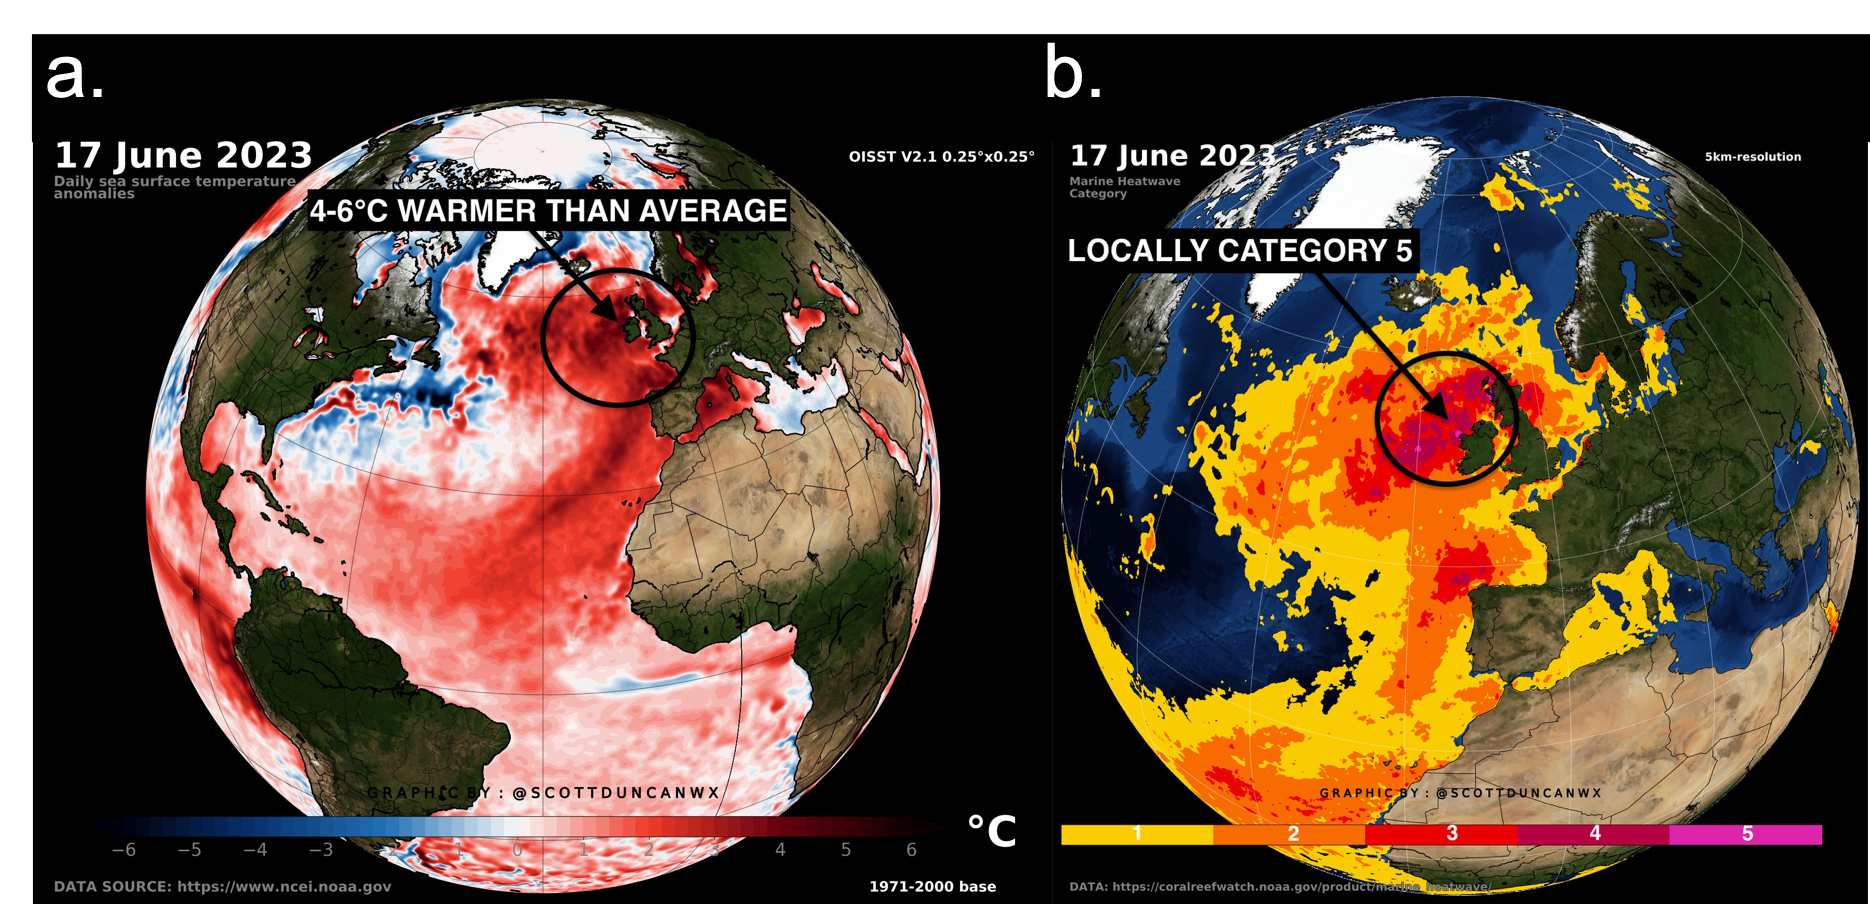
\includegraphics{02-Introduction/figures/marine_heatwaves.png}
\caption[Anomalies de températures et vagues de chaleurs extrêmes
identifiées au large des côtes dans l'est de l'Atlantique le 17 juin
2023]{Anomalies de températures et vagues de chaleurs extrêmes
identifiées au large des côtes dans l'est de l'Atlantique le 17 juin
2023. a. Anomalies de températures de surface supérieure à 2°C dans
l'ensemble de l'Atlantique Est avec localement des anomalies comprises
en +4 et +6°C au large des côtes irlandaises. b. Catégorisation des
vagues de chaleur dans l'Atlantique Est, avec des vagues de chaleur
allant du niveau 1 ``vague de chaleur modérée'' (i.e golfe de Gascogne)
jusqu'au niveau 5 ``au-delà de l'extrême'' au large de l'Irlande. ©
Infographie : Scott \textcite{Duncan}}\label{fig:intro3}
}
\end{figure}

Les activités anthropiques ont également induit des perturbations
considérables dans la chimie des océans. Les bassins océaniques agissent
comme des puits de carbone en transformant le CO\(_\text{2}\) en acide
carbonique via le processus de dissolution. Cette dissolution entraîne
une réduction du pH marin \autocite{ipcccarbonbiogeochem_2021}. Depuis
l'ère préindustrielle, on note une diminution du pH océanique, oscillant
initialement au-dessus de 8.1 pour se rapprocher de 8 actuellement soit
une acidification de 21\% \autocite{ipcccarbonbiogeochem_2021}. Cette
acidification a des répercussions notables sur les écosystèmes côtiers.
Notamment, elle affecte la capacité des organismes tels que les algues
coralligènes, les coraux et les bivalves à synthétiser leurs structures
calcaires \autocites[ ]{Chan_2013}[ ]{Kuffner_2008}{Zhao_2017}. La
modification de la composition chimique des océans peut se traduire
également par une diminution de la concentration en oxygène \autocites[
]{Schmidtko_2017}{Breitburg_2018}. Les zones hypoxiques ont des
conséquences majeures pour les organismes côtiers : une teneur en
oxygène plus faible compromet la croissance et les fonctions
reproductives des organismes les moins tolérants avec des conséquences
sur les communautés et le fonctionnement des écosystèmes
\autocite{Limburg_2020}.

Les écosystèmes côtiers subissent une augmentation constante de ces
multiples pressions \autocite{ipbes_2019}. Ces pressions opèrent à
différentes échelles spatiales et temporelles et génèrent des effets
complexes souvent cumulatifs, ce qui complique la compréhension et
surtout la prédiction de leurs impacts. L'évolution récente des
écosystèmes terrestres et marins \autocite{Carmona_2021}, dans le
contexte du changement climatique global, met en lumière la nécessité de
mise en place de mesures de préservation et de stratégies de gestion
durable. Sans interventions, ces écosystèmes pourraient atteindre un
seuil de dégradation au-delà duquel leur restauration deviendrait très
limitée, voire impossible \autocite{Palmer_2020}.

Les perturbations subies par les écosystèmes affectent directement les
communautés d'espèces qu'ils abritent. Pour appréhender pleinement les
conséquences de ces changements sur la structure et le fonctionnement
des écosystèmes côtiers, il est essentiel de saisir comment les
communautés y maintiennent leur équilibre. La section suivante se
penchera sur l'écologie des communautés, mettant en lumière l'importance
des espèces animales et végétales pour la résilience des écosystèmes
côtiers face aux pressions environnementales et anthropiques.

\clearpage

\hypertarget{ecologie-des-communautuxe9s}{%
\section{Ecologie des Communautés}\label{ecologie-des-communautuxe9s}}

\hypertarget{mesurer-et-interpruxe9ter-la-diversituxe9-des-espuxe8ces-dans-une-communautuxe9}{%
\subsection{Mesurer et Interpréter la Diversité des Espèces dans une \\
Communauté}\label{mesurer-et-interpruxe9ter-la-diversituxe9-des-espuxe8ces-dans-une-communautuxe9}}

Les communautés écologiques, définies comme l'ensemble des espèces
coexistant dans une zone géographique spécifique, sont caractérisées par
leur diversité spécifique et l'abondance respective de chaque espèce
\autocite{Vellend_2010}. Au niveau local, la diversité d'une communauté,
appelée diversité \(\alpha\) \autocite{Whittaker_1960}, se reflète par
exemple, dans le nombre d'espèces présentes (c.-à-d.~la richesse
spécifique). Lors de la comparaison des communautés entre plusieurs
sites, c'est-à-dire en évaluant la variabilité des communautés en termes
de composition et de structure (par exemple, les patrons de dominance en
termes d'abondance), les chercheurs évaluent la diversité \(\beta\)
\autocite{Whittaker_1972}. Une faible diversité \(\beta\) signifie que
les sites ont des communautés similaires, tandis qu'une valeur élevée
indique des différences marquées entre les communautés. Etudier la
diversité \(\beta\) est une manière pour les chercheurs d'appréhender
les changements environnementaux en cours, car ces changements
n'affectent pas nécessairement le nombre d'espèces présentes dans une
zone de manière consistante. En revanche, les effets de ces changements
sont visibles à toutes les échelles via la composition des communautés
\autocite{Dornelas_2023}.

Mesurer la diversité spécifique, ne permet pas d'appréhender l'ensemble
des facettes de la biodiversité. La biodiversité est caractérisée par
une multitude de facettes différentes, dont la diversité des lignées
évolutives (c.-à-d.~diversité phylogénétique), ou bien la diversité des
traits fonctionnels des espèces (c.-à-d.~diversité fonctionnelle)
\autocite{Bagousse-Pinguet_2019}. La diversité fonctionnelle est un
aspect important de la biodiversité à mesurer, puisque l'étude des
variations de cet aspect de la biodiversité permet de mieux comprendre
l'effet des perturbations sur le fonctionnement global des écosystèmes
\autocite{Mouillot_2013}.

L'écologie des communautés, champ disciplinaire dans lequel s'inscrivent
ces travaux de thèse, vise donc à comprendre les facteurs régissant la
diversité des communautés, tout en cherchant à en établir des principes
universels. Ainsi, pour comprendre ces facteurs, il est important de
décrire les changements de biodiversité à différentes échelles spatiales
et temporelles, et via différentes méthodes pour comprendre la
biodiversité \autocite{Dornelas_2023}.

\hypertarget{la-niche-uxe9cologique-un-cadre-explicatif-de-la-diversituxe9-des-communautuxe9s}{%
\subsection{La niche écologique : un cadre explicatif de la diversité
des \\
communautés}\label{la-niche-uxe9cologique-un-cadre-explicatif-de-la-diversituxe9-des-communautuxe9s}}

Alors que les mesures de diversité offrent des indications précieuses
sur la variabilité et la similarité des communautés d'un écosystème,
elles ne fournissent pas, à elles seules, un cadre explicatif des
mécanismes sous-jacents. Pour comprendre les facteurs qui façonnent ces
patrons de diversité, il est essentiel de se tourner vers la théorie des
niches. Cette dernière nous offre des outils et des perspectives pour
appréhender les rôles écologiques et les besoins environnementaux des
espèces, permettant ainsi d'expliquer les raisons pour lesquelles
certaines espèces coexistent tandis que d'autres sont exclues.

Joseph Grinnell dans son article fondateur a décrit le concept de niche
écologique \autocite{Grinnell_1917}. La niche écologique grinnellienne
peut être définie comme l'ensemble des conditions environnementales qui
permettent aux espèces de persister et de se reproduire
\autocite{Grinnell_1917}. Quelques années plus tard, Elton étendit le
concept de Grinnell en définissant la niche écologique comme ``la place
d'un animal dans l'environnement abiotique et sa relation aux sources de
nourriture et à ses ennemies'' \autocite{Elton_1927}. Aujourd'hui, la
définition de niche écologique la plus utilisée en écologie moderne est
la définition de Hutchinson qui décrit la niche écologique comme un
système de coordonnées qui permettent de décrire un hypervolume à
n-dimension (\textcite{Hutchinson_1957} ; Fig.~\ref{fig:intro4}). Cet
espace multidimensionnel compte une dimension pour chaque ressource
utilisée par l'espèce en question, ainsi qu'une dimension supplémentaire
pour chaque espèce interagissant avec elle \autocite{Hutchinson_1957}.
Hutchinson décrivit plus précisément deux types de niches : la niche
fondamentale, l'hypervolume qui décrit l'ensemble des conditions
favorables dans lesquelles une espèce peut exister, et la niche
réalisée, qui est un sous-ensemble de la niche fondamentale contrainte
par les interactions biotiques et la disponibilité environnementale
(p.~ex. contrainte de dispersion). La niche réalisée, accessible aux
écologues par le biais de mesures \emph{in situ}, est souvent perçue
comme tronquée, car les complexités inhérentes à la mesure exhaustive de
toutes les dimensions de la niche sur le terrain est difficle
(Fig.~\ref{fig:intro4} ; \textcite{Chevalier_2022}).

\begin{figure}
\hypertarget{fig:intro4}{%
\centering
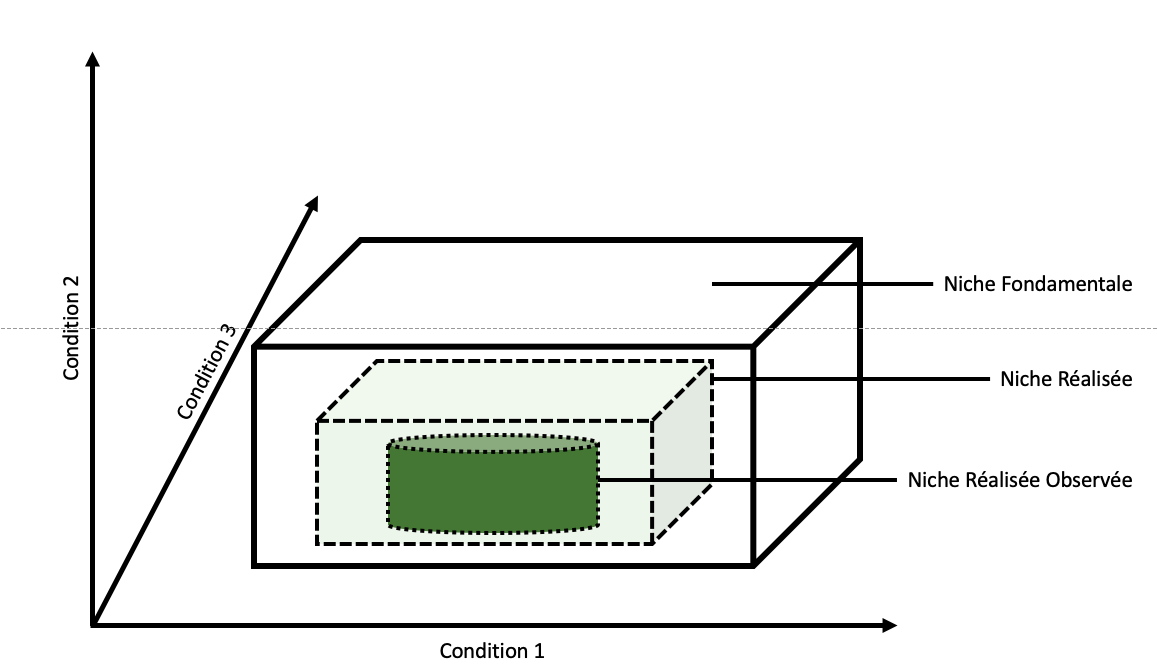
\includegraphics{02-Introduction/figures/hypervolume_niche.png}
\caption{Niche écologique d'une espèce marine virtuelle n'utilisant que
trois ressources.}\label{fig:intro4}
}
\end{figure}

Le concept de niche est utile aux écologues, car il permet de mesurer un
optimum écologique (c.-à-d.~les conditions où la \emph{fitness} de
l'espèce est maximal), d'estimer la largeur de la niche
(c.-à-d.~l'ensemble des conditions environnementales dans lesquelles une
espèce peut être trouvée), de mesurer le chevauchement des niches de
deux espèces (c.-à-d.~dans quelle mesure deux espèces peuvent être
trouvées dans des conditions similaires) \autocite{Chase_2003}.

Ainsi, la théorie des niches avance l'idée que la coexistence de
nombreuses espèces en un lieu spécifique résulte du fait que ces espèces
occupent des niches écologiques distinctes, présentant ainsi un faible
chevauchement. Ce constat conduit à une diversité \(\alpha\) élevée pour
ce site. En ce qui concerne la diversité \(\beta\), lorsque deux sites
possèdent des conditions environnementales semblables et que les niches
disponibles sont comparables entre elles, la diversité \(\alpha\) sera
faible. À l'opposé, si les conditions environnementales diffèrent entre
les deux sites, la diversification potentielle des niches entre ces
habitats pourrait entraîner une diversité \(\beta\) élevée.

\hypertarget{influence-des-espuxe8ces-inguxe9nieures-sur-la-structure-des-communautuxe9s}{%
\subsection{Influence des Espèces Ingénieures sur la Structure \\ des
Communautés}\label{influence-des-espuxe8ces-inguxe9nieures-sur-la-structure-des-communautuxe9s}}

Au sein d'une communauté, toutes les espèces qui la composent n'ont pas
la même influence sur sa structure et ses fonctions. Parmi l'ensemble
des espèces qui ont un rôle particulier pour structurer la communauté,
il est important dans le cadre de cette thèse de mentionner les espèces
ingénieures. Une espèce ingénieure est une espèce qui de par ses
structures, sa présence ou son comportement modifie la structure et le
fonctionnement de son habitat \autocite{Jones_1994}.

Il existe plusieurs catégories d'espèces ingénieures. Parmi ces
catégories, il est possible de distinguer les espèces fondatrices
\autocite{Dayton_1972} qui jouent un rôle crucial dans la structuration
des communautés, car leurs fortes abondances ou biomasses vont modifier
profondément l'environnement \autocite{Ellison_2019}. Leur importance
est d'autant plus marquée lorsque l'on reconnaît que bon nombre
d'espèces fondatrices sont responsables de la création d'habitats
biogéniques \autocites[ ]{Thomsen_2010}{Thomsen_2018}. Ces habitats
biogéniques, issus de la production biologique des organismes vivants,
ouvrent dans l'environnement de nouvelles niches écologiques, en
modifiant les ressources disponibles, influençant les flux de matière et
d'énergie, et peuvent abriter une multitude d'autres organismes,
induisant ainsi une augmentation de la biodiversité locale \autocites[
]{Bruno_2003}[ ]{Sunday_2017}{Romero_2015}.

En somme, les habitats biogéniques et les espèces qui les forment jouent
un rôle clé dans la réponse présente et future des écosystèmes marins
côtiers face aux changements globaux et impacts anthropiques \autocites[
]{Sunday_2017}[ ]{Harley_2006}{Bulleri_2018}. Leur étude est donc
critique d'un point de vue de la gestion et de la préservation des
écosystèmes, mais elle permet aussi de répondre à des questions
d'écologie fondamentale. Mieux comprendre le fonctionnement et la
réponse de ces habitats peut ainsi fournir des éclairages quant aux
processus qui promeuvent la biodiversité \autocite{Romero_2015}, aux
mécanismes de rétroaction qui stabilisent les écosystèmes
\autocite{Thomsen_2010}, ainsi que sur les liens entre biodiversité et
fonctionnement des écosystèmes \autocite{Hastings_2007}.

\hypertarget{la-disparition-des-habitats-bioguxe9niques}{%
\subsection{La Disparition des Habitats
Biogéniques}\label{la-disparition-des-habitats-bioguxe9niques}}

Les habitats biogéniques jouent un rôle essentiel dans la génération et
le maintien de la biodiversité et peuvent également servir de
sentinelles face aux changements environnementaux \autocites[
]{Roca_2016}[ ]{Nugues_2003}{Fredericq_2019}. Leur sensibilité à une
multitude de pressions, qu'elles soient d'origine anthropique ou
naturelle, en fait des indicateurs des changements environnementaux. Par
exemple, un déclin observé dans un herbier marin peut signaler une
dégradation de la qualité des eaux \autocite{Roca_2016}. De la même
manière, les coraux, avec leur sensibilité au stress thermique, sont des
témoins des effets du changement climatique
\autocite{Hoegh-Guldberg_1999}. Ainsi, la surveillance de l'état de
santé de ces habitats biogéniques peut nous fournir des informations
vitales sur les changements plus larges qui se produisent dans
l'écosystème.

Les habitats biogéniques sont de plus en plus menacés par les activités
humaines \autocite{Wernberg_2023}. En quarante ans, la grande barrière
de corail, le plus grand récif corallien au monde, a perdu près de la
moitié de sa superficie \autocite{Hughes_2015} et les herbiers marins
ont perdu dans le même temps plus de 30\% de leur superficie mondiale
\autocites[ ]{Waycott_2009}{Dunic_2021}. Les causes de la diminution de
superficie de ces habitats biogéniques sont multifactorielles et
reposent sur l'ensemble des pressions directes et indirectes décrites
précédemment. Dans les chapitres suivants, les termes \emph{ecosytem
engineer}, \emph{biogenic habitat} et \emph{foundation species} sont
ainsi utilisés indistinctement.

Cependant, cette disparition n'est pas immédiate, les habitats peuvent
passer par plusieurs stades de dégradation différents appelés dans la
suite de cette thèse ``état d'habitat''. Par exemple,
\textcite{Donovan_2018} identifie 5 états d'habitats de récifs
coralliens avec des degrés de biomasse de poissons, de couverture en
corail et de macroalgues différentes témoignant de différents degrés de
dégradation (c.-à-d.~un état non dégradé, trois états de transitions et
un état dégradé).

Les conséquences de la dégradation et de la disparition des habitats
biogéniques sont difficiles à anticiper du fait de leur importance au
sein des écosystèmes. La perte de ces habitats entraîne une cascade
d'événements dans l'écosystème. Sans ces habitats pour servir de zones
de frayère, de nourriture et de protection, de nombreuses espèces se
retrouvent vulnérables (p.~ex. \textcite{Hughes_2009}). Le déclin des
habitats biogéniques est ainsi devenu l'un des principaux moteurs du
déclin de la biodiversité \autocite{ipbes_2019}, bousculant la stabilité
des écosystèmes tout entiers. Ainsi, l'étude des habitats biogéniques
offre également des perspectives intéressantes pour le développement de
programmes pour sauvegarder les écosystèmes marins \autocite{Loh_2019}.
Il est donc important de mieux comprendre leur écologie et les impacts
qu'ils ont sur leurs communautés associées, ainsi que de caractériser
leurs états et leurs distributions à l'échelle globale. Caractériser
leurs états et leurs distributions présents et futurs nécessite entre
autres de développer des outils pour prédire les changements d'état que
subissent ou risque de subir ces habitats face aux changements
environnementaux \autocite{Wernberg_2023}. Cela nécessite notamment de
comprendre les dynamiques complexes que peuvent montrer ces écosystèmes
face à des pressions multiples et variées \autocite{Nystrom_2012}.

\hypertarget{dynamique-des-uxe9cosystuxe8mes-ruxe9sistance-ruxe9sillience-et-changement-de-ruxe9gime}{%
\subsection{Dynamique des Écosystèmes : Résistance, Résillience et \\
Changement de
Régime}\label{dynamique-des-uxe9cosystuxe8mes-ruxe9sistance-ruxe9sillience-et-changement-de-ruxe9gime}}

Les communautés écologiques sont des systèmes dynamiques,
continuellement influencés par une multitude de perturbations. Ces
dernières peuvent être qualifiées de ``pulse''quand ponctuelles sur de
courtes durées, ou de ``press'' quand leurs impacts se font ressentir
sur une période plus longue \autocites[ ]{Bender_1984}{Ryo_2019}. Leur
amplitude peut varier \autocite{Jentsch_2019}, entraînant des impacts
soit progressifs, soit soudains sur les écosystèmes et leurs communautés
(Fig.~\ref{fig:intro5} ; \textcite{Spake_2022}).

\begin{figure}
\hypertarget{fig:intro5}{%
\centering
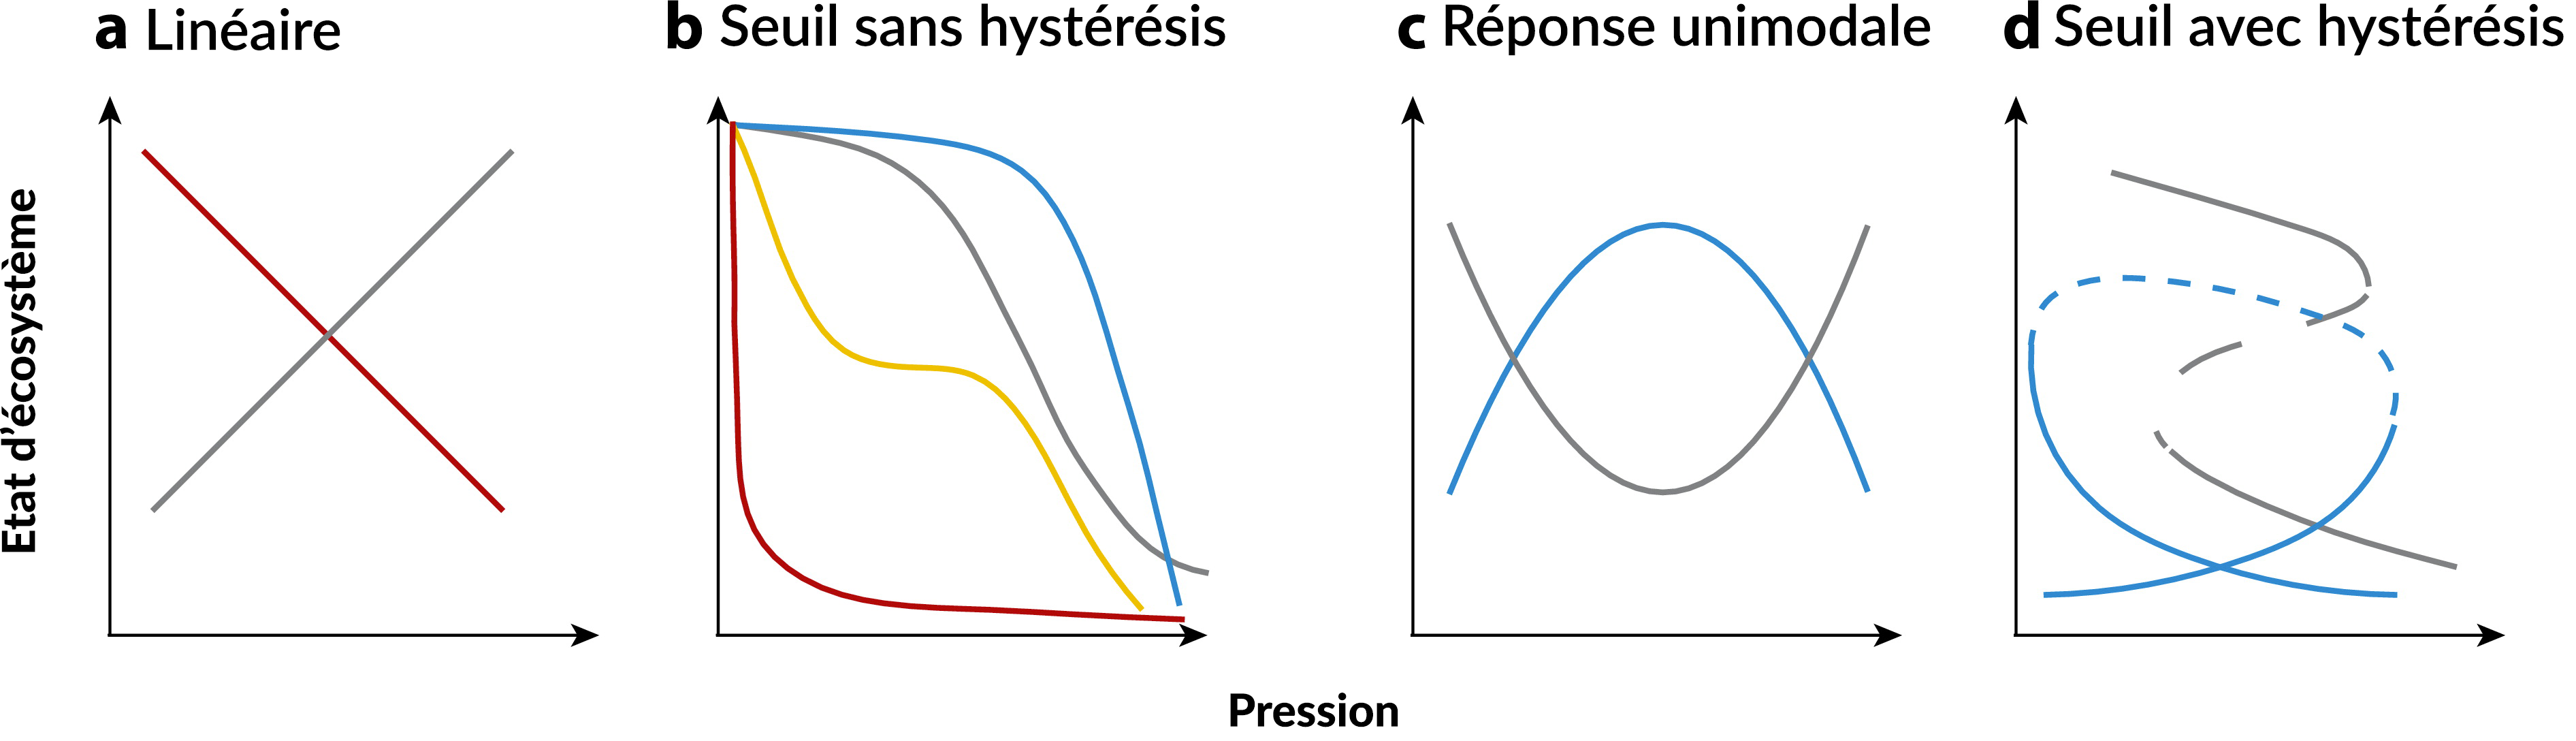
\includegraphics{02-Introduction/figures/ecosystem_responses.png}
\caption[Différentes réponses qu'un écosystème peut présenter face à des
pressions.]{Différentes réponses qu'un écosystème peut présenter face à des
pressions. Chaque courbe représente l'ensemble des points d'équilibre
potentiel d'un écosystème. Si ces graphes permettent de développer des
visions théoriques des dynamiques écologiques, ils sous-entendent une
simplification de la nature intrinsèquement changeante des écosystèmes.
a. Réponse linéaire b. Réponse avec seuil sans hystérésis c.~Réponse
unimodale d.~Réponse avec seuil et hystérésis. Dans ce cas, les courbes
en pointillés reflètent des points d'équilibre instable. Extrait de
\textcite{Spake_2022}}\label{fig:intro5}
}
\end{figure}

Face à ces perturbations, les communautés manifestent des propriétés de
résistance et de résilience (Fig.~\ref{fig:intro6}). La résistance
caractérise la capacité d'un système à maintenir sa structure et son
fonctionnement en présence de perturbations. Par exemple, dans les
écosystèmes marins, les mangroves démontrent une forte résistance aux
tempêtes tropicales grâce à leur système racinaire complexe
\autocite{Kazemi_2018}. La résilience, en revanche, fait référence à la
capacité d'un système à retourner à son état antérieur (supposément à
l'équilibre) suite à une perturbation. Il convient de noter que
différents écosystèmes, en fonction de la composition de leurs
communautés et de leurs propriétés intrinsèques, manifestent des
réponses variées aux perturbations.

\begin{figure}
\hypertarget{fig:intro6}{%
\centering
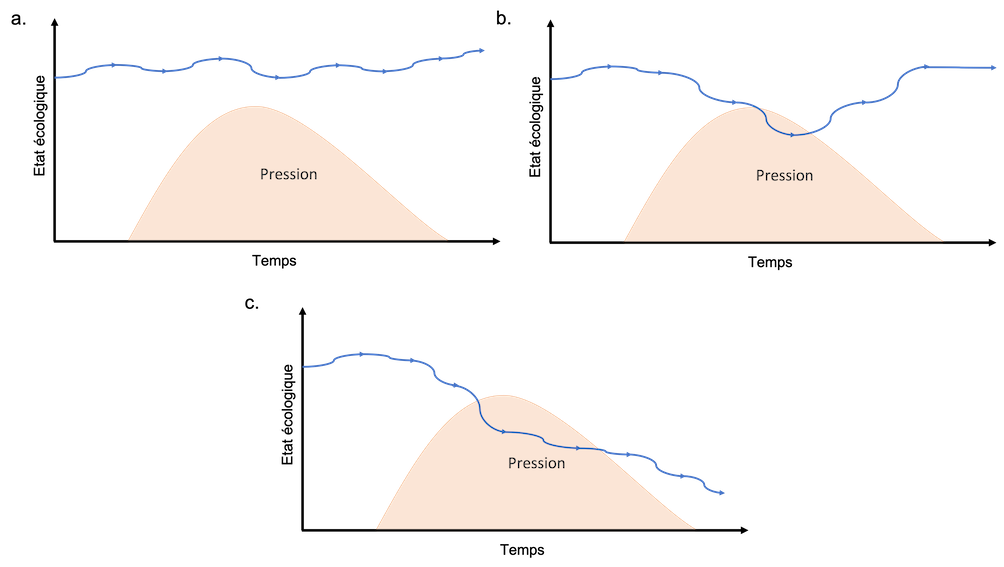
\includegraphics{02-Introduction/figures/resitance_resillience_schema.png}
\caption[Schéma décrivant la réponse théorique d'un écosystème à une
pression.]{Schéma décrivant la réponse théorique d'un écosystème à une
pression. a. L'écosystème présente une forte résistance à la pression
subite. b. L'écosystème présente une résistance moyenne à la pression,
mais une forte résilience. c.~L'écosystème présente à la fois une faible
résistance et résilience}\label{fig:intro6}
}
\end{figure}

Dans les cas où les pressions environnementales dépassent un certain
seuil, les écosystèmes peuvent subir des changements de régime
écologiques \autocite{Scheffer_2001}, passant à un nouvel état
écologique persistant, souvent considéré comme moins favorable
\autocites[ ]{Nystrom_2012}{Rocha_2015a}. Ces transitions peuvent être
linéaires ou non-linéaires \autocite{Scheffer_2015}, et peuvent
présenter des seuils au-delà desquels la restauration à l'état initial
est ardue, voire impossible (c.-à-d.~phénomène d'hystérésis,
Fig.~\ref{fig:intro5} d ; \textcite{Marzloff_2016} ;
\textcite{Johnson_2017} ; \textcite{Rocha_2018}). Ces changements de
régime ont été observés dans de nombreux écosystèmes : de la forêt à la
savane \autocite{Staver_2011}, de la toundra aux forêts boréales
\autocite{Scheffer_2012}, des récifs coralliens aux récifs dominés par
les macroalgues \autocite{McManus_2004}, ou bien encore l'effondrement
des pêcheries \autocite{Gardmark_2015}.

Comprendre les mécanismes sous-jacents à ces changements de régime est
essentiel pour élaborer des stratégies de gestion et de conservation
efficaces. En raison de la complexité et de l'interconnectivité des
facteurs impliqués, la prédiction et la prévention de ces changements
restent des défis considérables pour la recherche écologique
contemporaine.

\clearpage

\hypertarget{de-lobservation-in-situ-uxe0-la-moduxe9lisation}{%
\section{\texorpdfstring{De l'Observation \emph{In Situ} à la
Modélisation}{De l'Observation In Situ à la Modélisation}}\label{de-lobservation-in-situ-uxe0-la-moduxe9lisation}}

Une première approche pour étudier les mécanismes sous-jacents aux
changements de biodiversité réside dans l'expérimentation \emph{in situ}
ou en mésocosmes. Ces approches sont particulièrement utilisées en
écologie pour décrire des systèmes simplifiés à des échelles
spatio-temporelles réduites et composées de quelques espèces
\autocite{Witman_2015}. Ainsi, ces approches expérimentales ignorent
généralement les processus à plus larges échelles et les processus
régionaux qui régissent les patrons de biodiversités et biaisent notre
compréhension des phénomènes écologiques menant aux communautés
observées \autocite{Leibold_2017}. Augmenter les échelles des
expérimentations serait donc une solution à ce problème, mais effectuer
des manipulations expérimentales pour contrôler la biodiversité à
l'échelle de systèmes plus complexes (p.~ex. à l'échelle d'un écosystème
ou d'un biome) est tout simplement irréalisable
\autocite{Petersen2009_intro}.

L'utilisation de la modélisation apparaît comme une alternative
judicieuse pour surpasser ces problèmes d'échelles. Au cours du temps,
de nombreuses approches de modélisations ont été développées et sont
utilisées en écologie \autocite{Geary_2020}. Parmi l'ensemble des
approches, certaines nécessitent une description complète des mécanismes
écologiques en jeu et permettent par exemple d'étudier le comportement
d'un écosystème sous différents scénarios, d'autres à partir de données
parcellaires permettent d'inférer par exemple les niches
environnementales réalisées de diverses espèces et enfin, les modèles
conceptuels permettent de formaliser ou de développer des cadres
théoriques du fonctionnement des écosystèmes avec très peu de données
(voir Fig. 1 dans \textcite{Geary_2020} pour les différents cas d'usage
des différents types de modèles et leurs besoins respectifs en données).
De par leur diversité, les modèles permettent d'inférer des processus
aux échelles pertinentes pour comprendre les règles qui régissent les
patrons de diversités observés dans les écosystèmes
\autocite{Leibold_2017}. Ainsi, dans le contexte global de l'écologie
des communautés, la modélisation est un outil de choix pour mieux
comprendre le fonctionnement des écosystèmes dans leur ensemble
\autocite{Edgar_2016}.

\hypertarget{impacts-de-la-ruxe9volution-digitale-sur-la-recherche-en-uxe9cologique}{%
\subsection{Impacts de la Révolution Digitale sur la Recherche en
Écologique}\label{impacts-de-la-ruxe9volution-digitale-sur-la-recherche-en-uxe9cologique}}

Les évolutions rapides en écologie et dans d'autres domaines de la
recherche, tant d'un point de vue théorique qu'appliquées, ont été
rendues possibles par les développements grandissant de l'électronique
et de l'informatique. Un des premiers changements technologiques majeurs
dans les années 1970 concerne la sortie grand public du microprocesseur
comme l'Intel 4004 (Fig.~\ref{fig:intro7}). Les microprocesseurs ont
révolutionné le monde de l'informatique puisque pour la première fois
l'ensemble des composants électroniques d'un processeur furent
miniaturisés pour tenir dans un seul boîtier, engendrant un gain de
place considérable, augmentant la vitesse de calcul et une diminution de
la consommation énergétique. Ce changement technologique a permis la
démocratisation de l'informatique et l'apparition de l'ordinateur
personnel, rendant l'informatique plus accessible au monde
universitaire, et notamment aux écologues.

\begin{figure}
\hypertarget{fig:intro7}{%
\centering

\includegraphics{02-Introduction/figures/Intel_C4004.jpg}
\caption[Processeur Intel 4004 commercialisé en 1971]{Processeur Intel 4004 commercialisé en 1971. © Photographie :
Thomas \textcite{Nguyen}}\label{fig:intro7}
}
\end{figure}

Dans le même temps, les développements théoriques (p.~ex. théorie des
niches \autocite{Hutchinson_1957}, théorie de la biogéographie insulaire
\autocite{MacArthur_1967}, théorie des communautés écologiques
\autocite{Vellend_2017}, théorie des métacommunautés
\autocite{Leibold_2018}) ont fait passer progressivement l'écologie des
communautés d'une science descriptive à une science
hypothético-déductive où différentes hypothèses ont pu être testées à
l'aide de modèles statistiques, univariées et/ou multivariées
\autocite{Legendre_2012}. Grâce à la puissance de calcul apportée par
l'essor de l'informatique, de nouvelles méthodes d'analyses de données
ont été mises au point et c'est ainsi qu'en 1979 un ouvrage en deux
tomes regroupant l'ensemble des méthodologies statistiques
multidimensionnelles adaptées aux données écologiques a vu le jour
\autocites[ ]{Legendre_1979a}{Legendre_1979b}.

L'essor de l'électronique et de l'informatique a également permis
d'apporter de nouveaux outils aux écologues pour l'observation des
écosystèmes de la planète. Ainsi, depuis les années 1960 et le début du
programme Landsat \autocite{Wulder_2019}, le nombre de programmes
spatiaux pour l'observation de la Terre à l'aide de satellites, n'a
cessé d'augmenter et il est aujourd'hui possible de dénombrer plusieurs
centaines de satellites d'observation actuellement en orbite \autocites[
]{Tatem_2008}{Anderson_2018}. L'essor de l'internet à la fin des années
1990 a également marqué un nouveau tournant pour les sciences en
général. Ce réseau informatique a permis de connecter les chercheurs du
monde entier, facilitant la collaboration et la diffusion des
connaissances dans le monde entier. Un bon exemple de projet
collaboratif à grande échelle concerne les plateformes \emph{Global
Biodiversity Information Facility} (\emph{GBIF}) ou \emph{Ocean
Biodiversity Information System} (\emph{OBIS}), qui ont pour but de
collecter des données sur l'occurrence et la distribution des espèces
pour contrôler l'état de la biodiversité à large échelle. Cet essor du
numérique est également corrélé avec celui des programmes de suivis de
la biodiversité à long terme \autocite{Buckley_2021b} et des programmes
de suivis de sciences participatives tels que \emph{eBird}
\autocite{Wood_2011b}, \emph{iNaturalist} \autocite{Unger_2021} ou bien
encore le programme \emph{Reef Life Survey} \autocite{Edgar_2014b}.

L'écologie rentre donc dans le monde du big data, présentant de
nouvelles perspectives et problématiques aux chercheurs
\autocite{Farley_2018}. Face à cette prolifération de données,
l'écologie des communautés doit désormais adopter des outils numériques
sophistiqués issus des sciences des données pour identifier des motifs
sous-jacents ou pour tester de nouvelles hypothèses. Ainsi, il est d'une
importance croissante de former les nouvelles générations d'écologues
aux outils numériques et aux méthodologies de la science des données.
Grâce à ces connaissances, ils pourraient faire émerger de nouvelles
techniques et de nouveaux paradigmes pour mieux comprendre et décrire la
biodiversité dans le contexte du changement global.

\hypertarget{des-muxe9thodes-dordination-aux-moduxe8les-de-distribution-despuxe8ces-une-exploration-des-approches-quantitatives-en-uxe9cologie}{%
\subsection{Des Méthodes d'Ordination aux Modèles de Distribution \\
d'Espèces : Une Exploration des Approches Quantitatives en \\
Écologie}\label{des-muxe9thodes-dordination-aux-moduxe8les-de-distribution-despuxe8ces-une-exploration-des-approches-quantitatives-en-uxe9cologie}}

Comme établi précédemment, les communautés se caractérisent par leur
dynamisme intrinsèque, rendant leur étude complexe. Face à cette
complexité, une panoplie d'outils numériques et mathématiques a vu le
jour. Les sections suivantes fourniront une présentation de certains de
ces outils, en particulier ceux utilisés dans cette thèse, à savoir: (1)
les méthodes d'ordination, essentielles pour déchiffrer les patrons
écologiques; (2) les méthodes de groupements, conçues pour détecter des
discontinuités au sein de données écologiques; enfin (3) les modèles de
distribution d'espèces, qui se base sur la théorie des niches pour
expliquer et prédire la distribution spatiale des espèces.

\hypertarget{ordinations}{%
\subsubsection{Ordinations}\label{ordinations}}

Les ordinations classiquement utilisées en écologie numérique telles
l'\emph{Analyse en Composante Principale} (\emph{PCA}), l'\emph{Analyse
de Correspondance} (\emph{CA}) ou le \emph{Positionnement
multidimensionnel} (\emph{MDS}) sont des techniques d'analyse
multidimensionnelles qui reposent sur l'idée de trouver une façon de
factoriser la matrice de composition d'espèces d'une certaine façon en
fonction de l'espace des dimensions souhaitées (Euclidien pour la
\emph{PCA}, Chi-carré pour la \emph{CA}, et divers selon la fonction de
distance appliquée pour la \emph{MDS}) pour résumer les informations
contenues dans la matrice de communauté \autocites[
]{Legendre_2012}{Udell_2015}.

De nombreuses avancées ont été faites dans le champ de recherche active
qu'est celui de la réduction de la dimensionnalité des données. De
nouvelles méthodes basées sur les graphes de voisinage
(Fig.~\ref{fig:intro8}) ont vu le jour ces dernières années comme
\emph{Isomap} \autocite{Tenenbaum_2000}, \emph{t-SNE}
\autocite{vanderMaaten_2008} ou bien encore \emph{UMAP}
\autocite{McInnes_2020}. Le principe de l'ensemble de ces méthodes est
de construire des graphes dans l'espace multidimensionnel originel des
données en connectant les points ``proches'' les uns aux autres par des
arêtes. L'idée générale est de déterminer quels sont les points (et donc
les communautés) qui sont le plus semblables (proches dans l'espace
multidimensionnel) ou dissemblables (éloignés dans l'espace
multidimensionnel). Les méthodes basées sur des graphes de voisinage
projettent les points dans un espace en plus faible dimension, tout en
cherchant à préserver les relations de voisinage entre les points
décrits par le graphe dans l'espace multidimensionnel. Pendant des
années, ces méthodes numériquement plus gourmandes en ressources et/ou
sans package facilement utilisable étaient rarement utilisées par les
écologues. Cependant, ces méthodes commencent à faire leur apparition
dans la boîte à outils des écologues des communautés \autocites[
]{Roberts_2020}{Milosevic_2022}.

\clearpage

\begin{figure}
\hypertarget{fig:intro8}{%
\centering
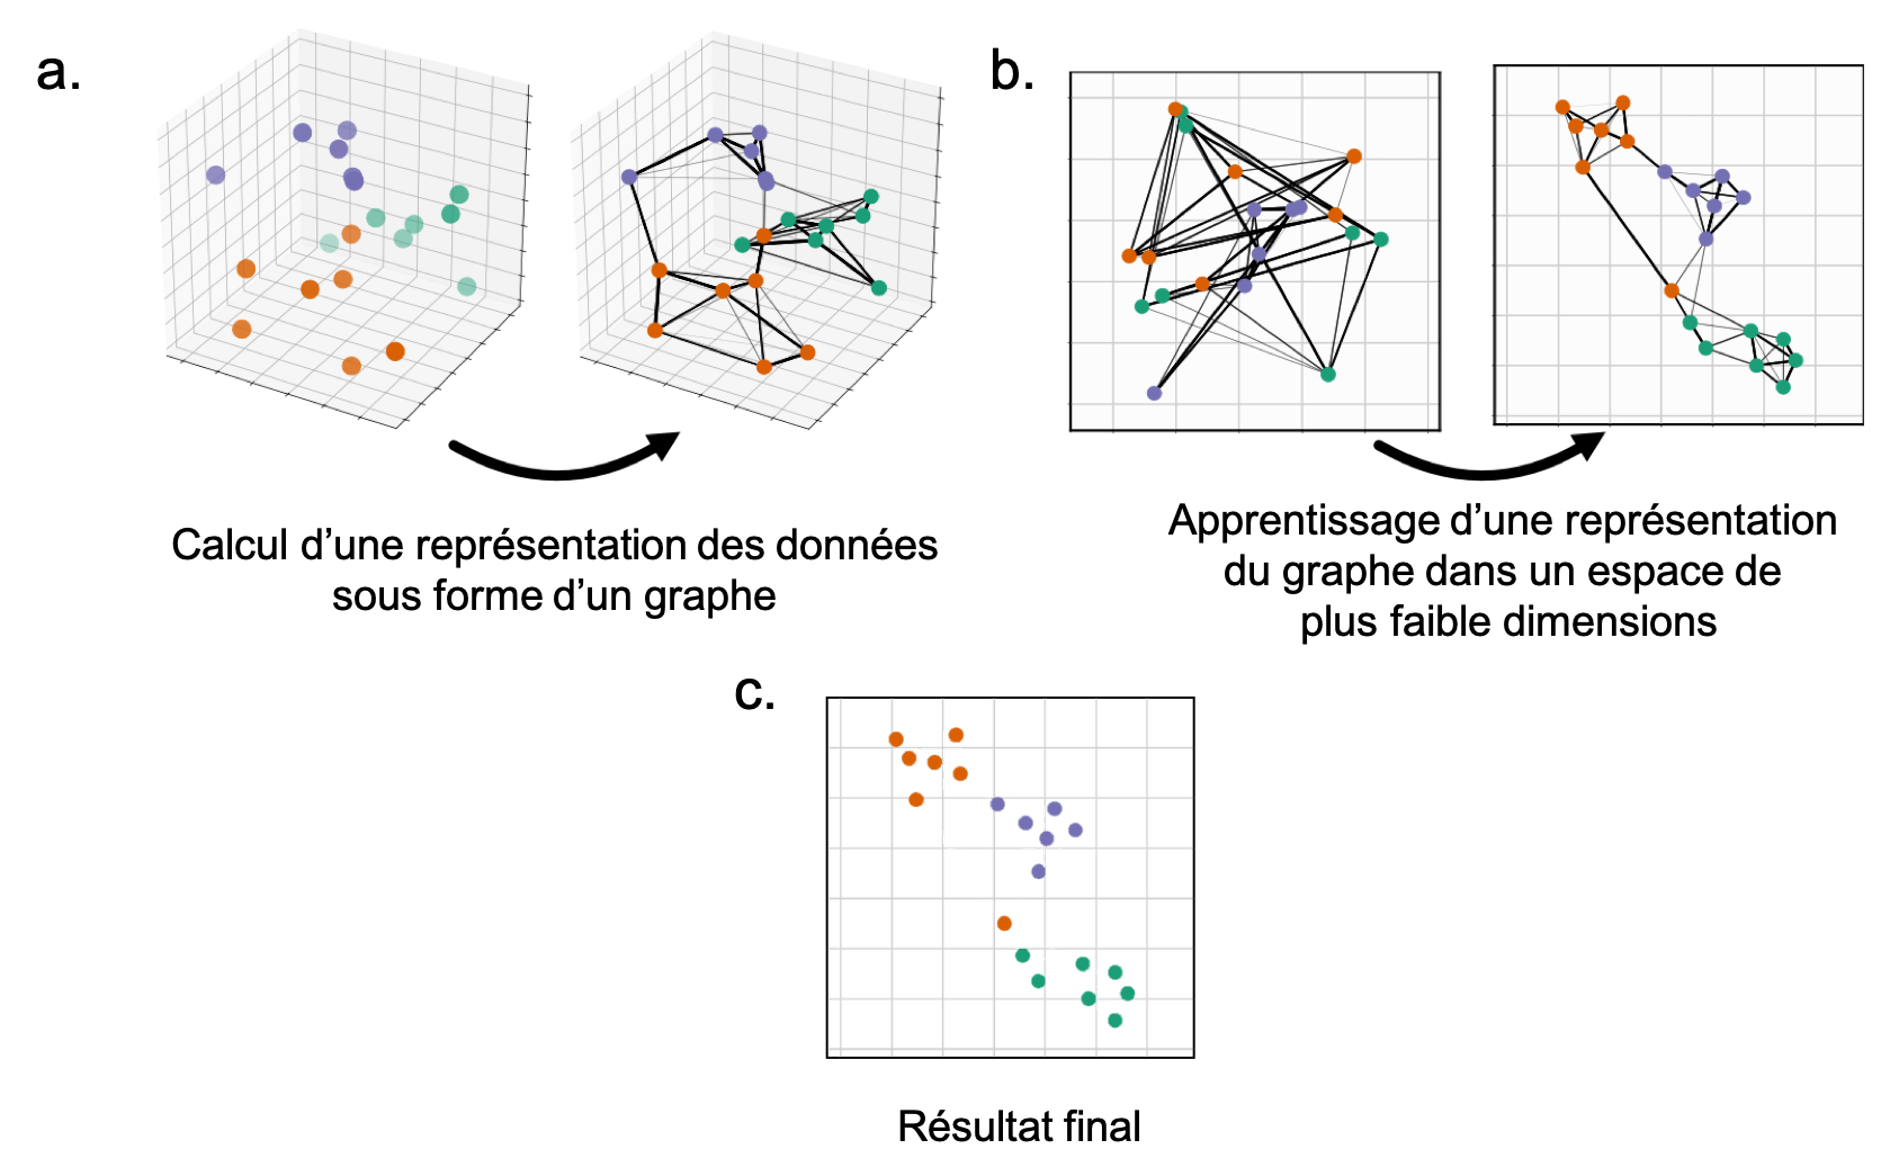
\includegraphics{02-Introduction/figures/neighbor_graph_dimension_reduction_technic.png}
\caption[Schéma du principe de fonctionnement d'une méthode de réduction
de dimension basée sur les graphes de voisinages.]{Schéma du principe de fonctionnement d'une méthode de réduction
de dimension basée sur les graphes de voisinages. a. Calcul d'un graphe
de voisinage dans l'espace multidimensionnel originel des données. b.
Apprentissage d'une représentation de ce graphe dans un espace de plus
faible dimension. c.~Projection des observations dans l'espace en plus
faible dimension. Adapté de
\textcite{McInnes2018umap-software}}\label{fig:intro8}
}
\end{figure}

\hypertarget{sec:introclustering}{%
\subsubsection{Méthodes de Groupement en
Ecologie}\label{sec:introclustering}}

D'une manière générale, l'être humain cherche à catégoriser les objets
qui le côtoient afin de mieux les décrire. Avant de les nommer, il nous
est nécessaire de les regrouper en catégories distinctes, qui ne sont
rien d'autre que des abstractions utiles à notre appréhension du monde.
Ainsi, il faut pouvoir développer des définitions, des heuristiques ou
bien encore des méthodes pour identifier des groupes distincts dans un
milieu qui, bien que parfois discret, est généralement continu
\autocite{Legendre_2012}.

L'usage des méthodes de groupement reste très fréquent en écologie des
communautés. Ce type de méthodes permet entre autres de définir des
groupes d'espèces ayant les mêmes traits \autocite{Mouillot_2021}, ou
partageant les mêmes patrons spatiaux de distribution
\autocite{Pang_2023}, d'identifier des zones similaires par rapport à
leur composition spécifique \autocite{Legendre_2012}, d'identifier des
écorégions dans l'océan global \autocite{Sonnewald_2020} ou bien encore
d'identifier des patrons spatiaux dans des réseaux écologiques
\autocite{Ohlsson_2020}.

Parmi les méthodes fréquemment utilisées en écologie, il est possible de
citer entre autres les méthodes hiérarchiques, comme celle de Ward ou du
groupement à liens simples ou complets, et non hiérarchiques comme le
\emph{k-means} \autocite{Legendre_2012}. L'avantage de ces méthodes est
leur facilité de compréhension. Cependant, le groupement hiérarchique à
liens simples est sensible au bruit contenu dans les données
\autocite{Legendre_2012} alors que les autres méthodes ont pour
contraintes de n'identifier que des groupes sphériques.

Pour contourner ces deux problèmes, d'autres méthodes ont été
développées en sciences des données. Ces algorithmes de groupement issu
d'une famille appelée ``\emph{Density-Based Clustering}'' imposent une
autre contrainte aux groupes à identifier : ces derniers doivent
contenir un certain nombre d'observations avant de pouvoir être déclarés
comme étant un cluster à part entière (c'est-à-dire qu'ils doivent être
denses) tout en permettant à des observations trop éloignées de ces
groupes de n'être assigné à aucun d'entre eux (observations considérées
alors comme bruit ; \textcite{Kriegel_2011}). Ainsi, la contrainte de la
forme des groupes est relaxée tout en permettant de définir des groupes
dépourvus d'observations bruitées. Bien que certaines de ces méthodes
aient été développées dès la fin du 20ème siècle \autocites[
]{Ester_1996}{Ankerst_1999}, elles n'ont été utilisées que très
récemment en écologie dues à leur complexité en coût de calcul et leur
difficulté à paramétrer (voir \textcite{Ohlsson_2020} et
\textcite{Sonnewald_2020}).

\hypertarget{moduxe8les-de-distribution-despuxe8ces}{%
\subsubsection{Modèles de Distribution
d'Espèces}\label{moduxe8les-de-distribution-despuxe8ces}}

Les modèles de distribution d'espèces sont des outils largement utilisés
en écologie pour comprendre, prédire et cartographier la distribution
spatiale d'une espèce en fonction des conditions environnementales
\autocite{Guisan_2000}. Enracinés dans la théorie des niches, ces
modèles reposent sur l'identification des relations entre les
occurrences connues (ou l'abondance) d'une espèce et un ensemble de
variables environnementales à ces localités, qui décrivent alors la
niche réalisée de l'espèce \autocite{Guisan_2017}.

Il est possible de classer les modèles de distribution d'espèces en deux
catégories : les modèles dits ``mécanistiques'' et les modèles dits
``corrélatifs''. Les modèles ``mécanistiques'' reposent sur une
représentation explicite des mécanismes associés aux variations de
biodiversité (p.~ex. augmentation du métabolisme de l'espèce en
condition de stress) \autocite{Kearney_2010}, alors que les modèles
``corrélatifs'' s'appuient sur les corrélations observées entre
l'environnement et les occurrences/abondance des espèces étudiées sans
mettre en évidence les mécanismes sous-jacents \autocite{Briscoe_2023}.

Les modèles mécanistiques modélisent la distribution des espèces ou des
communautés \autocite{Harfoot_2014}, à l'aide d'équations
différentielles qui intègrent explicitement les processus physiologiques
de réponses aux variations environnementales \autocite{Kearney_2009}.
Cependant, l'une des critiques principales de la modélisation
mécanistique réside dans sa difficulté à être appliquée pour les
espèces, communautés ou écosystèmes peu étudiés, du fait de la nécessité
de traduire des hypothèses écologiques en équations
\autocite{Evans_2015} et de l'acquisition de données physiologiques sur
les espèces étudiées \autocite{Gandra_2015}.

Les modèles corrélatifs quant à eux sont bien plus utilisés en écologie
des communautés pour modéliser la distribution des espèces
(\emph{Species Distribution Models} ou \emph{SDM}, en anglais). Basés
sur des modèles statistiques tels que les régressions linéaires, ces
modèles trouvent des relations corrélatives entre les données
environnementales et les données d'occurrence (ou d'abondance) d'une
espèce \autocite{Guisan_2017}. Toutefois, les relations observées entre
les occurrences et les données environnementales sont souvent
non-linéaires et peuvent être mieux modélisées grâce à des modèles
additifs généralisés \autocite{Guisan_2002}, ou à l'aide de modèles de
\emph{Machine Learning} \autocite{Elith_2006}. Cette variété d'approches
de modélisation s'est enrichie avec l'apport de nouvelles de données qui
ont permis de mieux caractériser la niche écologique des espèces en
prenant en compte leurs traits \autocite{Pollock_2012} ou bien les
relations phylogénétiques entre différentes espèces
\autocite{Ives_2011}. L'ensemble de ces techniques de modélisation ont
permis de faire des progrès majeurs en écologie notamment en permettant
de mieux comprendre la niche écologique réalisée des espèces, en créant
des cartes de distribution d'espèces menacées pour aider à la mise en
place de plans de gestion \autocite{Franklin_2013}, en prédisant les
zones d'expansion d'espèces envahissantes \autocite{Mainali_2015}, ou en
étudiant les changements de distribution d'espèces et des patrons de
diversités associés selon différents scénarios de changement climatique
\autocite{Araujo_2019}.

Néanmoins, cette approche ne permet pas de modéliser l'ensemble d'une
communauté puisque, en considérant les espèces comme indépendantes les
unes des autres, elle ne prend pas en compte la nature multivariée des
données en écologie \autocites[ ]{Warton_2015}{Ovaskainen_2017a}. Pour
pallier à cet écueil, \textcite{Ferrier_2006} proposèrent plusieurs
approches : (1) ``\emph{grouper, puis prédire}'', (2) ``\emph{prédire
puis grouper}'' et enfin (3) ``\emph{prédire et grouper simultanément}''
(Fig.~\ref{fig:intro9}).

\begin{figure}
\hypertarget{fig:intro9}{%
\centering
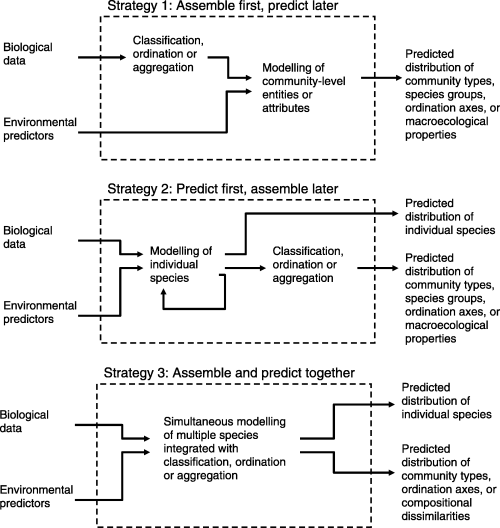
\includegraphics{02-Introduction/figures/ferriers_strategies.png}
\caption[Stratégies de modélisations de distribution d'espèces.]{Stratégies de modélisations de distribution d'espèces.
\textcite{Ferrier_2006}}\label{fig:intro9}
}
\end{figure}

Pour résumer les différentes approches proposées par
\textcite{Ferrier_2006}, la première consiste à utiliser des techniques
de classification ou d'ordination (voir Sec.~\ref{sec:introclustering})
pour d'abord caractériser différents types de communautés d'espèces
avant d'ensuite prédire leurs distributions et leurs déterminants. La
seconde approche consiste à modéliser séparément chaque espèce de la
communauté, puis les prédictions de chaque modèle sont agrégées par des
méthodes de classification ou d'ordination. Une variante de cette
approche consiste à modéliser chaque espèce indépendamment des autres
puis à compiler les prédictions de ces modèles pour prédire les
assemblages d'espèces présents, sans considérer les potentielles
interactions interspécifiques (\emph{stacked-SDM} en anglais;
\textcite{Pollock_2020}). Enfin, la dernière approche propose de prédire
toutes les espèces et de les agréger en une communauté en une seule
étape via des approches de modélisation multidimensionnelles, qui
prennent en compte les patrons de co-occurence entre espèces
\autocite{Warton_2015}. Chacune de ces approches présente des forces et
des faiblesses différentes \autocites[ ]{DAmen_2017}[
]{Pollock_2020}{Norberg_2019}.

Ainsi l'approche ``\emph{prédire et grouper simultanément}'' est selon
\textcite{Ferrier_2006} la plus polyvalente, permettant de prédire la
distribution de chaque espèce individuellement tout en capturant de
manière adéquate les propriétés macroécologiques des communautés. Plus
difficile à mettre en place, cette approche a récemment connu un regain
d'intérêt grâce au développement de nouvelles approches pour estimer la
distribution jointe de toutes les espèces d'une communauté à l'aide
d'outils statistiques accessibles aux écologues \autocites[
]{Warton_2015}[ ]{Hui_2016}[ ]{Ovaskainen_2017a}[ ]{Niku_2019}[
]{Chiquet_2021}{Pichler_2020}. Ces \emph{Joint Species Distribution
Models} (\emph{jSDM}) se proposent de modéliser, à l'aide d'une
distribution multidimensionnelle (c.-à-d.~normale multivariée), toutes
les espèces d'une communauté en fonction de différents prédicteurs, tout
en prenant en compte l'effet de prédicteurs potentiels (c.-à-d.~non
inclus dans le modèle) grâce à un système de variables latentes
\autocite{Warton_2015}.

\pagebreak

Si cette approche ``\emph{prédire et grouper simultanément}'' paraît
prometteuse, son implémentation n'est pas sans défi \autocites[
]{Poggiato_2021}{DAmen_2017}. D'autres approches méthodologiques ont
aussi des atouts qu'il convient d'examiner, notamment lorsqu'il s'agit
de faire le lien avec la gestion des écosystèmes \autocites[
]{DAmen_2017}{Pollock_2020}. L'approche ``\emph{grouper, puis prédire}''
a par exemple été utilisée pour explorer les déterminants à large
échelle des patrons biogéographiques en milieu marin
\autocite{Belanger_2012}. Dans ce contexte, cette thèse s'appuiera sur
une diversité de méthodes complémentaires pour répondre aux objectifs
suivants.

\clearpage

\hypertarget{contexte-objectifs-de-cette-thuxe8se}{%
\section{Contexte \& Objectifs de cette
Thèse}\label{contexte-objectifs-de-cette-thuxe8se}}

Les habitats biogéniques marins, dont les forêts d'algues, les herbiers
marins et les récifs coralliens, représentent des piliers fondamentaux
pour la sauvegarde de la biodiversité marine et le bon fonctionnement
des écosystèmes côtiers \autocite{ipbes_2019}. Malheureusement, leur
intégrité est mise à mal par une myriade de pressions, qu'elles soient
d'origine anthropique ou naturelle \autocite{ipbes_2019}. Afin de
garantir la préservation de la biodiversité marine et la pérennité des
fonctions écologiques essentielles des zones côtières, une compréhension
approfondie de ces habitats est impérative. Cette compréhension passe
par la caractérisation des états d'habitats et des facteurs qui
régissent leur distribution, mais aussi par une meilleure description de
leur dynamique et des interrelations complexes que ces habitats
biogéniques entretiennent avec la biodiversité qu'ils abritent
(Fig.~\ref{fig:intro10}).

\begin{figure}
\hypertarget{fig:intro10}{%
\centering
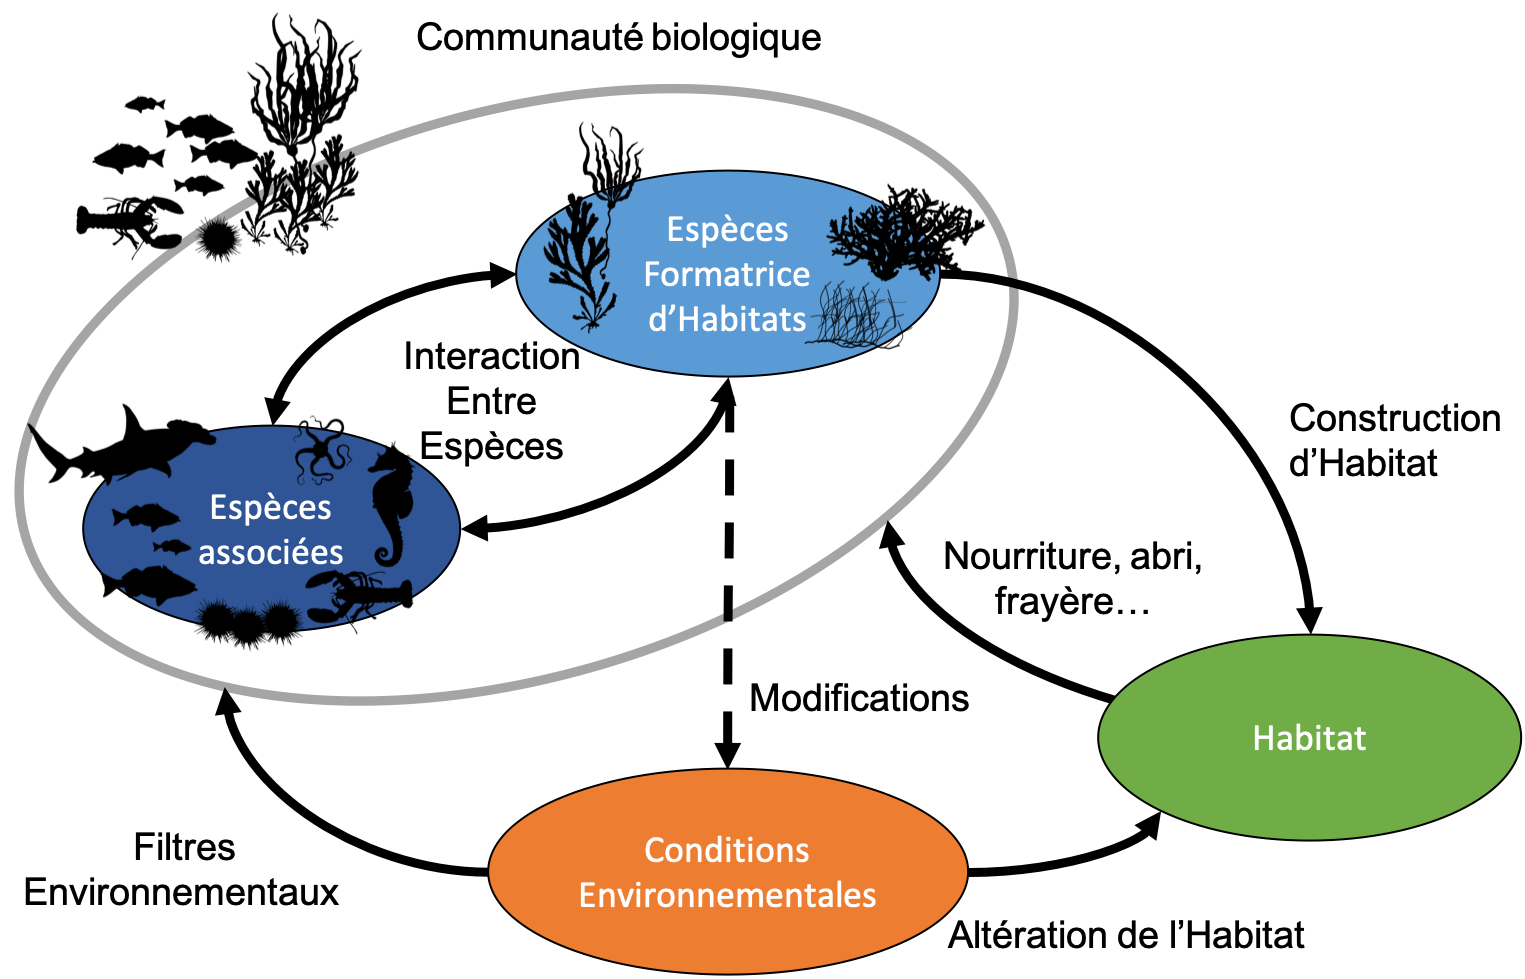
\includegraphics{02-Introduction/figures/research_framework.png}
\caption[Schéma illustrant les interactions majeures entre les habitats
benthiques, la faune et les conditions environnementales]{Schéma illustrant les interactions majeures entre les habitats
benthiques, la faune qui y est associée et les conditions
environnementales. Cadre de pensée dans lequel s'inscrit cette thèse.
Adapté d'après \textcite{Marzloff_2022}}\label{fig:intro10}
}
\end{figure}

L'ambition première de cette thèse est d'améliorer notre compréhension
globale du fonctionnement des habitats biogéniques côtiers. Elle vise à
caractériser le rôle des habitats biogéniques et de leurs différents
états sur la biodiversité environnante, mais aussi à éclairer notre
vision des transitions potentielles d'habitats au sein des
environnements benthiques côtiers (Fig.~\ref{fig:intro10}). Pour mener à
bien ces objectifs, ce travail de thèse a été divisé en trois chapitres
qui utilisent deux approches distinctes (Fig.~\ref{fig:intro11}).

Dans le premier chapitre, j'ai testé l'approche ``\emph{prédire et
grouper simultanément}'', via l'usage de \emph{jSDM}, pour comprendre
les règles d'assemblage d'espèces et les patrons de biodiversité
associés à deux habitats caractéristiques des écosystèmes benthiques
côtiers de Bretagne. En particulier, l'objectif était de comprendre et
prédire les réponses des communautés de macroinvertébrés associées à ces
habitats le long de gradients environnementaux. Pour ce faire, j'ai
développé une méthodologie d'évaluation des performances des différentes
prédictions réalisables par un \emph{jSDM} que j'ai appliqué à un jeu de
données issu de séries temporelles de 8 ans couvrant l'ensemble du
littoral breton (\href{http://rebent.ifremer.fr}{rebent.fr}). Grâce à
cela, j'ai pu identifier les avantages et les limites de différentes
structures de \emph{jSDM} qui intègrent différentes sources
d'information (phylogénie, trait, information sur la communauté
accompagnatrice) quant à leur capacité à expliquer et prédire des
patrons de biodiversité locaux et leur déploiement à large échelle.

Dans les chapitres deux et trois, j'ai testé une approche se basant sur
les états d'habitats biogéniques comme proxy pour étudier la
biodiversité, dans une démarche ``\emph{grouper puis, prédire}''. Dans
le second chapitre, j'ai ainsi cherché à créer une typologie d'habitats
benthiques biogéniques en me basant sur des données de couverture
d'habitats, collectées grâce à un programme de sciences participatives
déployé à l'échelle du globe
(\href{https://reeflifesurvey.com}{reeflifesurvey.com}). J'ai développé
une nouvelle méthodologie de \emph{Machine Learning} pour classifier ces
données d'observation en alliant une méthode de réduction de dimensions
basée sur les graphes de voisinage et un algorithme de groupement basé
sur la densité. A l'aide d'outils d'interprétation de modèles de
\emph{Machine Learning}, j'ai pu comprendre quelle était la composition
de ces types d'habitats, étudier leur distribution spatiale et
temporelle et leur diversité à l'échelle globale.

\pagebreak

Dans le troisième chapitre, j'ai qualifié les niches environnementales
des états d'habitats biogéniques découverts dans le chapitre précédent
par une approche de modèles de distribution d'espèces. J'ai identifié
l'influence relative de différentes pressions anthropiques et variables
environnementales sur la distribution de ces états d'habitats. Les
résultats de ces travaux ont montré que plusieurs états d'habitats ont
des niches environnementales similaires. Ces travaux ont permis ainsi de
mettre en évidence des zones et des conditions environnementales où
l'apparition de différents états d'habitats est plus probable.

\begin{figure}
\hypertarget{fig:intro11}{%
\centering
\includegraphics{02-Introduction/figures/Resumé_these.png}
\caption{Schéma illustrant les travaux réalisés dans le cadre de ce
travail de thèse.}\label{fig:intro11}
}
\end{figure}

\printbibliography[heading=subbibintoc, title={Bibliographie}]
\end{refsection}